\section{Adsorption material test - water purification}
In this study the capacity of five different materials were tested with regards to their ability to adsorb heavy metal ions (copper and zinc) in polluted water over a defined time interval. The tested material were concrete, zeolites, goethite, ion exchange resins and active carbon. They were tested one by one using SpinChem\textsuperscript{\textregistered}’s patented rotating bead reactors (RBR). To analyze how the pH changed during the purification process a pH test was construct for concrete and goethite. 
\subsection{Method}
The materials were sieved (300-700 $\mu$m) and washed in distilled water before studied. The concentration of copper and zinc ions were measured by the analytic methods FAAS and ICP-OES (see Analytical methods). To measure the capacity to adsorb metal ions of the mentioned materials, 20 ml material was added to a SpinChem\textsuperscript{\textregistered} RBR S221. A reference sample was taken before the loaded reactor was lowered into the reaction vessel V211 containing 200 ml polluted water and then rotated at 700 rpm. In the first set, all materials were investigated separately and samples were taken at three time points, 30, 60 and 120 minutes. The experiment was repeated for concrete, zeolites and goethite with the time interval: 10 seconds, 1, 3, 7, 15 and 30 minutes. At each time point, a sample of 10 ml was taken wi3th a syringe and filtered into falcon tubes. For each ml sample, 10 $\mu$l 7 M nitric acid was added in the falcon tubes and sent to FAAS analysis. 

After reviewing the results from the FAAS analysis, goethite was chosen for ICP-OES analyze to further investigate its capacity to adsorb heavy metal ions. For this test, a larger RBR was used along with a larger amount of the material. 50 ml material was added to the RBR S331 in the reaction vessel V311 which contained 1.2 l polluted water, before rotating at 700 rpm. Nine samples including a reference sample were taken at the given times of 10 seconds, 1, 3, 7, 15, 30, 60 and 120 minutes. The samples were collected in the same fashion as the previously described.

To examine how concrete and goethite affect pH during the reaction, 20 ml material was added to the RBR S221 in the reaction vessel V211 containing 200 ml polluted water and rotated at 700 rpm. pH was measured with litmus paper during a two hour period (figure \ref{fig:pH}).

\subsection{Analytical methods}
After the experiments, the concentrations of heavy metal ions (copper and zinc) were measured using two different analytical methods called Flame Atomic Absorption Spectroscopy (FAAS) and Inductively Coupled Plasma Optical Emission Spectroscopy (ICP-OES). The principle behind FAAS is that a heated flame, in the atomizer, excites the electrons in the atoms, making the electrons migrate into higher orbitals for a few nanoseconds. The amount of energy absorbed for this transition to occur is very specific for each heavy metal ion. This amount of energy is measured with a detector that translates the energy into concentrations [1]. The analytical technique inductively coupled plasma optical emission spectroscopy (ICP-OES) produce excited atoms and ions by using the inductively coupled plasma at a wavelength that is specific for a certain type of heavy metal ion. The analytical methods has different detection limits depends on the type of machine. ICP-OES can in general detect lower levels of concentration, compared to FAAS analysis. ICP-OES can also analyze several metal ions at the same measurement while FAAS can only analyze one type of metal ion at a time [2], [3].

 
\subsection{Results}
The capacity of the different materials to adsorb metal ions in polluted water over time was analysed. The metal ions, zinc and copper, were measured with the analytic methods FAAS and ICP-OES described above.

The FAAS analysis revealed that the concentration of zinc ions decreased for all materials after 30 minutes (figure \ref{fig:faasZinc}). The same reference sample was used for all the materials. Goethite was the material that decreased the concentration of zinc ions the most after 120 minutes. Concrete was the material determined to have the lowest adsorption capacity for zinc ions. Between 30 and 120 minutes, the concentration of zinc ions increased when using concrete. The FAAS analysis revealed that the concentration of copper ions decreased for all materials except zeolites after 120 minutes (figure \ref{fig:faasCopper}). Between 60 and 120 minutes, the concentration of copper ions increased for concrete.  


\begin{figure}[H]
    \centering
    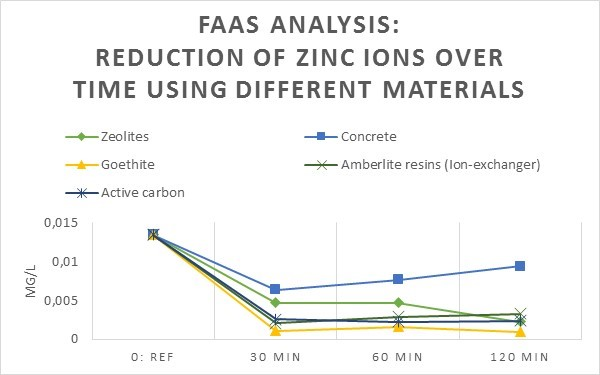
\includegraphics[width=0.7\textwidth]{faasZinc}
    \caption{The concentrations of zinc ions (mg/l) in polluted water measured at four time points (0, 30, 60 and 120 minutes) for the five different materials using the analytic method FAAS.}
	\label{fig:faasZinc}
\end{figure}


\begin{figure}[H]
    \centering
    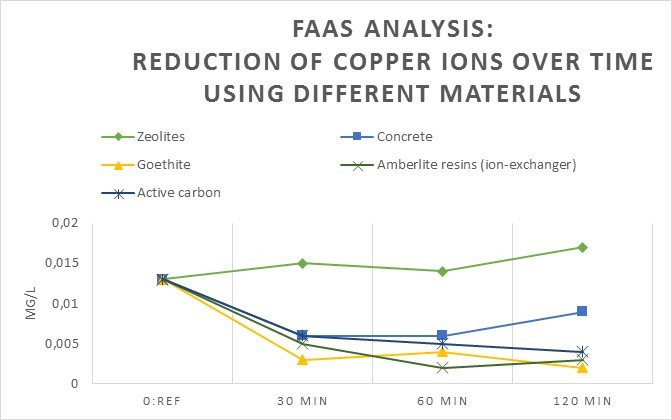
\includegraphics[width=0.7\textwidth]{faasCopper}
    \caption{The concentrations of copper ions (mg/l) in polluted water measured at four time points (0, 30, 60 and 120 minutes) for the five different materials using the analytic method FAAS.}
	\label{fig:faasCopper}
\end{figure}

The experiment was repeated for zeolites, concrete and goethite but with shorter time interval and more frequent sampling. The concentration of zinc ions were analysed with FAAS. After 10 seconds the concentration of zinc ions had increased for all materials (figure \ref{fig:faasZincShort}). After 30 minutes, goethite was the material that had adsorb most zinc ions. With concrete as material, the concentration of zinc ions started to increase after 7 minutes.


\begin{figure}[H]
    \centering
    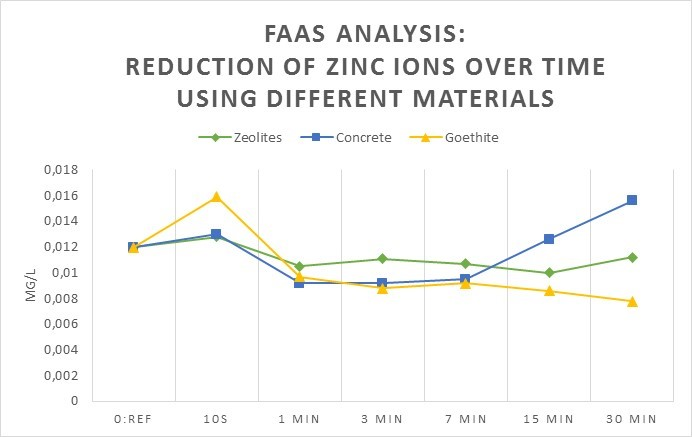
\includegraphics[width=0.7\textwidth]{faasZincShort}
    \caption{The concentrations of zinc ions (mg/l) measured at seven time points, including the reference for the three materials, zeolites, concrete and goethite, using the FAAS analysis.}
	\label{fig:faasZincShort}
\end{figure}

The result for the ICP-OES analysis with samples from the experiment with goethite showed that the concentration of copper ions decreased for up to 15 minutes. Between 15 and 120 minutes the concentration was stable at 0.02 mg/l (figure \ref{fig:icpoesCopper}). The result for the concentration of zinc ions with goethite displayed negative values but it indicated a decrease for up to 3 minutes and then stabilized (figure \ref{fig:icpoesZinc}).

\begin{figure}[H]
    \centering
    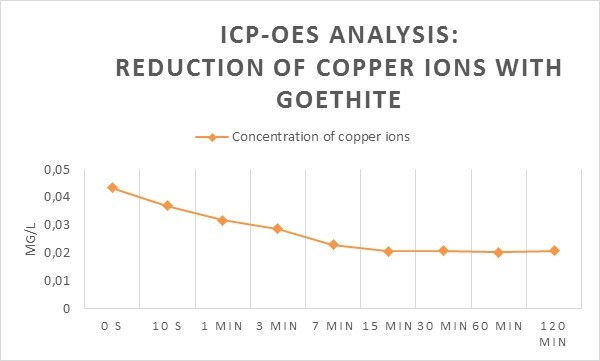
\includegraphics[width=0.7\textwidth]{icpoesCopper}
    \caption{The concentration of copper ions (mg/l) measured at nine time points, including the reference sample using goethite and analysed with ICP-OES.}	\label{fig:icpoesCopper}
\end{figure}


\begin{figure}[H]
    \centering
    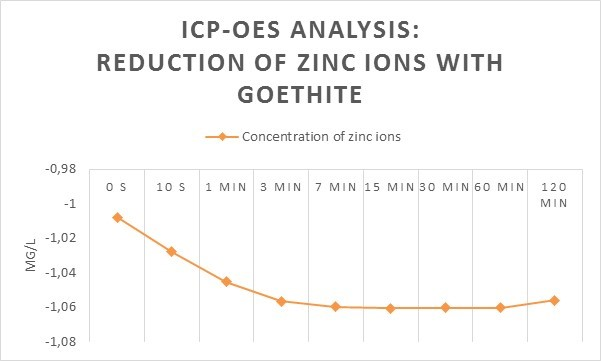
\includegraphics[width=0.7\textwidth]{icpoesZinc}
    \caption{The concentration of zinc ions (mg/l) measured at nine time points, including the reference sample using goethite and analysed with ICP-OES.}
	\label{fig:icpoesZinc}
\end{figure}

The result for the pH measurements of concrete and goethite in polluted water containing metal ions showed to be stable at pH 5 for goethite during the whole time interval (figure \ref{fig:pH}). For concrete, the pH rose from 5 to 10 the first 5 minutes and later rose to 12.


\begin{figure}[H]
    \centering
    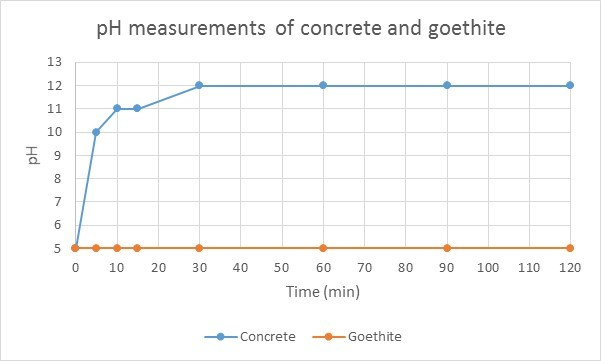
\includegraphics[width=0.7\textwidth]{pH}
    \caption{pH measurements with litmus paper of concrete and goethite at eight time points, including the reference, in polluted water containing metal ions.}
	\label{fig:pH}
\end{figure}

\subsection{Discussion}
A part of this project was to use SpinChem\textsuperscript{\textregistered}’s patented RBR and evaluate the capacity of different materials to adsorb metal ions in solution over time. The results from the FAAS analysis showed that all materials adsorb zinc ions after 120 minutes but had different capacities (figure \ref{fig:faasZinc}). The concentration of zinc ions in the solution decreased more during the first 30 minutes and then the levels were quite stable. This could be due to that the materials became saturated and was not able to adsorb more zinc ions. The results also showed that concrete seemed to leak out zinc ions back to the solution after 30 minutes. This might be because the bond between zinc ions and concrete is weak and unstable or it favours other ions in the solution. The results for copper ions showed that all materials except zeolites were able to adsorb first 30 minutes (figure \ref{fig:faasCopper}). As for the materials to adsorb zinc ions the result showed a similar pattern and after 30 minutes the concentration of copper ions were quite stable. This could also be due to saturation as in the case with the zinc ions. It seems like the zeolite was not able to adsorb copper ions and might have greater affinity for other particles. 

Since the result for zinc ions showed a large decrease during the first 30 minutes for all materials, we chose to repeat the experiment with zeolite, concrete and goethite with shorter time intervals along with more frequent sampling. The result was unexpected, the concentration of zinc ions were quite unchanged during the 30 minutes (figure \ref{fig:faasZincShort}). This could be due to that the standard that was prepared for the FAAS analysis might have had higher starting concentrations compared to our samples and therefore no conclusion could be drawn. 

After FAAS analysis we decided to continue the study with goethite since it had the highest capacity to adsorb zinc and copper ions (figure \ref{fig:faasZinc}, 7, \ref{fig:faasZincShort}). We repeated the experiment in larger scale (1,2 l) and chose to analyse with ICP-OES. The result showed that the reduction of copper ions in the solution decreased more during the first 15 minutes and then the concentration became stable at 0,02 (figure \ref{fig:icpoesCopper}). Goethite seemed to become saturated after 15 minutes and therefore not able to adsorb more copper ions. The result for the concentration of zinc ions in the solution showed negative values of the concentration but displayed a similar pattern as the results for the copper ions (fig \ref{fig:icpoesZinc}). Goethite seemed to be able to adsorb copper ions during the first \ref{fig:faasCopper} minutes before becoming saturated. The negative values could be due to errors of measurement in the ICP-OES machine. Comparing the analytical methods FAAS and ICP-OES, both methods seemed to display a decrease of copper and zinc ions in the polluted water for goethite the first 30 minutes and then stabilized. Both methods seemed to indicate that goethite became saturated after 30 minutes and it is unnecessary to continue with the purification process for 120 minutes. Since both methods gave different reference values even though it was the same pollutant water it is difficult to compare the concentrations from the results. The pH measurements for concrete and goethite gave different results. For goethite, the pH level was stable around 5 during the whole time interval (figure \ref{fig:pH}). This might be due to that the material bind to other ions or release ions that does not affect the pH. The pH rose from 5 to 12 during the entire time interval. The large increase of the pH could be that concrete leaked ions that affected the pH. The material could also bind hydrogen ions that affect the pH. 

In summary, goethite seems to have the best capacity to adsorb zinc and copper ions compared to the other materials tested. Concrete does not seem to bind the metal ions permanently, since the concentrations increases with time. Since the concentration of metal ions in the solution was already low to begin with, the method for analyzment did not seemed to be good enough as an analytical tool for this study and in the future a more sensitive method should be used. 


